% $Header: /home/vedranm/bitbucket/beamer/solutions/generic-talks/generic-ornate-15min-45min.en.tex,v 90e850259b8b 2007/01/28 20:48:30 tantau $

\documentclass{beamer}
  
% This file is a solution template for:

% - Giving a talk on some subject.
% - The talk is between 15min and 45min long.
% - Style is ornate.



% Copyright 2004 by Till Tantau <tantau@users.sourceforge.net>.
%
% In principle, this file can be redistributed and/or modified under
% the terms of the GNU Public License, version 2.
%
% However, this file is supposed to be a template to be modified
% for your own needs. For this reason, if you use this file as a
% template and not specifically distribute it as part of a another
% package/program, I grant the extra permission to freely copy and
% modify this file as you see fit and even to delete this copyright
% notice. 


\mode<presentation>
{
  \usetheme{Hannover}
  \usecolortheme{crane}

  \setbeamercovered{transparent}
  % or whatever (possibly just delete it)
}
\usepackage{amsmath}

\usepackage[english]{babel}
% or whatever

\usepackage[latin1]{inputenc}
% or whatever

\usepackage{times}
\usepackage[T1]{fontenc}
% Or whatever. Note that the encoding and the font should match. If T1
% does not look nice, try deleting the line with the fontenc.


\title[Governing Equations] % (optional, use only with long paper titles)
{Governing Equations of \\ Classical Gas Dynamics}

\subtitle
{Characteristics form and Simple Waves} % (optional)

\author[Manuel Diaz] % (optional, use only with lots of authors)
{Manuel Diaz\inst{1} }
% - Use the \inst{?} command only if the authors have different
%   affiliation.

\institute[National Taiwan University] % (optional, but mostly needed)
{
  \inst{1}%
  National Taiwan University\\
  Institute of Applied Mechanics}
%  \and
%  \inst{2}%
%  Department of Theoretical Philosophy\\
%  University of Elsewhere}
% - Use the \inst command only if there are several affiliations.
% - Keep it simple, no one is interested in your street address.

\date[August 31th, 2011] % (optional)
{August 31th, 2011 / Weekly Meeting}

\subject{Talks}
% This is only inserted into the PDF information catalog. Can be left
% out. 



% If you have a file called "university-logo-filename.xxx", where xxx
% is a graphic format that can be processed by latex or pdflatex,
% resp., then you can add a logo as follows:

% \pgfdeclareimage[height=0.5cm]{university-logo}{university-logo-filename}
% \logo{\pgfuseimage{university-logo}}



% Delete this, if you do not want the table of contents to pop up at
% the beginning of each subsection:
%-------------------------------------------------------------------
%\AtBeginSubsection[]
%{
%  \begin{frame}<beamer>{Outline}
%    \tableofcontents[currentsection,currentsubsection]
%  \end{frame}
%}
%--------------------------------------------------------------------

% If you wish to uncover everything in a step-wise fashion, uncomment
% the following command: 

%\beamerdefaultoverlayspecification{<+->}


\begin{document}

\begin{frame}
  \titlepage
\end{frame}

\begin{frame}{Outline}
  \tableofcontents
  % You might wish to add the option [pausesections]
\end{frame}


% Since this a solution template for a generic talk, very little can
% be said about how it should be structured. However, the talk length
% of between 15min and 45min and the theme suggest that you stick to
% the following rules:  

% - Exactly two or three sections (other than the summary).
% - At *most* three subsections per section.
% - Talk about 30s to 2min per frame. So there should be between about
%   15 and 30 frames, all told.

\section{Euler Equations}

\subsection{Conservation Form}

\begin{frame}{CONSERVATION FORM}
  \begin{itemize}
   \item Euler Equations expresed in classical conservation form:
  \end{itemize}
  \begin{eqnarray}
    \fra\frac{y}{x}\partial x
    &&\frac{\partial{\rho}}{\partial{t}}+\frac{\partial{{\rho}{u}}}{\partial{x}}=0, \\
    &&\frac{\partial{{\rho}u}}{\partial{t}}+\frac{\partial{({\rho}{u^2}+p})}{\partial{x}}=0, \\
    &&\frac{\partial{\rho}e_T}{\partial{t}}+\frac{\partial{({\rho}{u}e_T+pu})}{\partial{x}}=0, \\
    &&\frac{\partial{\rho}s}{\partial{t}}+\frac{\partial{{\rho}{u}s}}{\partial{x}}\geq 0
  \end{eqnarray} 
\end{frame}

\begin{frame}{VECTOR NOTATION}{Vectors of conserved quantities}
  \begin{itemize}
   \item Define the Vectors of conserved quantities:
  \end{itemize}
  \begin{equation}
    \vec{u} = \begin{bmatrix}
      {\rho} \\
      {\rho}{u} \\
      {\rho}{e_T}
    \end{bmatrix}=\begin{bmatrix}
      u_1\\ 
      u_2\\ 
      u_3
      \end{bmatrix}
  \end{equation}
  \begin{equation}
   \vec{f} = \begin{bmatrix}
      {\rho}{u} \\
      {\rho}{u^2}+p \\
      ({\rho}{e_T}+p)u
    \end{bmatrix}=\begin{bmatrix}
      f_1\\ 
      f_2\\ 
      f_3
      \end{bmatrix}
  \end{equation}
\end{frame}

\subsection{- Vector Notation} 

\begin{frame}{VECTOR NOTATION}{of the conservation equation}
  \begin{itemize}
   \item By using the vectors of conserved quantities, we can express in a very compact form the Euler Equations:
  \end{itemize}
  \begin{equation}
   \frac{\partial{\vec{u}}}{\partial{t}}+\frac{\partial{\vec{f}}}{\partial{x}}=0
  \end{equation}
  \begin{itemize}
  \item But we know:
  \end{itemize}
  \begin{equation}
  \vec{f}(\vec{u})
  \end{equation}
\end{frame}

\begin{frame}{VECTOR NOTATION}
  \begin{itemize}
   \item The by the chain rule
  \end{itemize}
  \begin{equation}
   \frac{\partial{\vec{u}}}{\partial{x}}=\frac{\partial\vec{f}}{\partial\vec{u}}\frac{\partial{\vec{u}}}{\partial{x}}
  \end{equation}
  where
  \begin{equation}
    \frac{\partial{\vec{u}}}{\partial{x}}=\begin{bmatrix}
    \frac{\partial{f_1}}{\partial{u_1}} & \frac{\partial{f_1}}{\partial{u_2}} & \frac{\partial{f_1}}{\partial{u_3}}\\ 
    \frac{\partial{f_2}}{\partial{u_1}} & \frac{\partial{f_2}}{\partial{u_2}} & \frac{\partial{f_2}}{\partial{u_3}}\\ 
    \frac{\partial{f_3}}{\partial{u_1}} & \frac{\partial{f_3}}{\partial{u_2}} & \frac{\partial{f_3}}{\partial{u_3}}
    \end{bmatrix}
  \end{equation}
\end{frame}

\subsection{- Matrix Notation} 

\begin{frame}{MATRIX NOTATION}
  \begin{itemize}
   \item To simplify, we call the Jacobian Matrix: A
  \end{itemize}
  \begin{equation}
    \frac{\partial{\vec{u}}}{\partial{t}}+A\frac{\partial{\vec{u}}}{\partial{x}}=0
  \end{equation}
  Computing A we obtain:
  \begin{equation}
   A=\begin{bmatrix}
    0 & 1 & 0\\ 
    \frac{\gamma-3}{2}u^2 & (3-\gamma)u & \gamma-1\\ 
    {\gamma}{u}e_T+(\gamma-1)u^3 & {\gamma}e_T-\frac{3}{2}(\gamma-1)u^2 & {\gamma}u
    \end{bmatrix}
  \end{equation}
\end{frame}

\subsection{Primitive Variable Form}

\begin{frame}{THE MATERIAL DERIVATE}
  \begin{itemize}
   \item The Primite variable from is not commonly used in gasdynamics. 
   \item The Primite variables are those flow variable that we can dyrectly measure.
   \item This is a lagrangean description of the Euler Equations.
  \end{itemize}
The Material Derivate:
  \begin{equation}
   \frac{D}{Dt}=\frac{\partial}{\partial{t}}+u\frac{\partial}{\partial{x}}
  \end{equation}
\end{frame}

\begin{frame}{PRIMITIVE VARIABLE FORM}
  \begin{itemize}
   \item The material derivate is rate of change a long the pathlines.
   \item Using the material derivate we rewrite the Euler Equations as:
  \end{itemize}
  \begin{eqnarray}
    &&\frac{D\rho}{Dt}+\rho\frac{\partial{u}}{\partial{x}}=0 \\
    &&\frac{Du}{Dt}+\frac{1}{\rho}\frac{\partial{p}}{\partial{x}}=0 \\
    &&\frac{Dp}{Dt}+{\rho}a^2\frac{\partial{u}}{\partial{x}}=0 \\
    &&\frac{Ds}{Dt}\geq 0
  \end{eqnarray}
\end{frame}

\begin{frame}{VECTOR-MATRIX FORM}
  \begin{itemize}
   \item Define the vector of primitive variables:
  \end{itemize}
The Material Derivate:
  \begin{equation}
   \vec{w}=\begin{bmatrix}
   \rho\\ 
   u\\ 
   p
   \end{bmatrix}
  \end{equation}
\end{frame}

\begin{frame}{VECTOR-MATRIX FORM}
  \begin{itemize}
   \item Then primitive form of the Euler equations can be written as:
  \end{itemize}
  \begin{equation}
   \frac{\partial{\vec{w}}}{\partial{t}}+C\frac{\partial{\vec{w}}}{\partial{x}}=0
  \end{equation}
Where:
  \begin{equation}
   C=\begin{bmatrix}
    u & \rho & 0\\ 
    0 & u & \frac{1}{\rho}\\ 
    0 & {\rho}a^2 & u
    \end{bmatrix}
  \end{equation}
\end{frame}

\begin{frame}{IMPORTANT RELATIONS}
  \begin{itemize}
   \item Relations between A and C: First notice that:
  \end{itemize}
  \begin{equation}
    d\vec{u}=Qd\vec{w}
  \end{equation}
where
  \begin{equation}
    Q=\frac{d\vec{u}}{d\vec{w}}=\begin{bmatrix}
    1 & 0 & 0\\ 
    u & \rho & 0\\ 
    \frac{1}{2}u^2 & {\rho}u & \frac{1}{\gamma-1}
    \end{bmatrix} 
  \end{equation}
\end{frame}

\begin{frame}{IMPORTANT RELATIONS}
  \begin{itemize}
   \item Relations between A and C: Or:
  \end{itemize}
  \begin{equation}
    d\vec{w}=Qd^{-1}\vec{u} 
  \end{equation}
where
  \begin{equation}
    Q^{-1}=\frac{d\vec{w}}{d\vec{u}}=\begin{bmatrix}
    1 & 0 & 0\\ 
    -\frac{1}{\rho}u & \frac{1}{\rho} & 0\\ 
    1/2(\rho-1)u^2 & -(\rho-1)u & \gamma-1
    \end{bmatrix}
  \end{equation}
\end{frame}

\begin{frame}{IMPORTANT RELATIONS}
  \begin{itemize}
   \item Relations between A and C:
  \end{itemize}
  \begin{eqnarray}
   &&Q\frac{\partial{\vec{w}}}{\partial{t}}+AQ\frac{\partial{\vec{w}}}{\partial{x}}=0 \\
   &&\frac{\partial{\vec{w}}}{\partial{t}}+Q^{-1}AQ\frac{\partial{\vec{w}}}{\partial{x}}=0 \\
   &&\frac{\partial{\vec{w}}}{\partial{t}}+C\frac{\partial{\vec{w}}}{\partial{x}}=0
  \end{eqnarray}
  \begin{itemize}
   \item In other words, A and C are similar matrices!
  \end{itemize}
\end{frame}

\begin{frame}{VECTOR-MATRIX FORM}
  \begin{itemize}
   \item Let's look again to the Primitive Variable Form:
  \end{itemize}
  \begin{equation}
   \frac{\partial{\vec{w}}}{\partial{t}}+C\frac{\partial{\vec{w}}}{\partial{x}}=0
  \end{equation}
Where:
  \begin{equation}
   C=\begin{bmatrix}
    u & \rho & 0\\ 
    0 & u & \frac{1}{\rho}\\ 
    0 & {\rho}a^2 & u
    \end{bmatrix}
  \end{equation}
\end{frame}

\subsection{The Characteristic Form}

\begin{frame}{CHARACTERISTIC FORM}
  \begin{itemize}
   \item Matrix C is a diagonizable and therefore:
   \item $Q_c^{-1}CQ_c=\Lambda$
  \end{itemize}
Where:
  \begin{eqnarray}
    &&Q_c^{-1}=\begin{bmatrix}
    1 & \rho/2a & -\rho/2a\\ 
    0 & 1/2 & 1/2\\ 
    0 & {\rho}a/2 & -{\rho}a/2
    \end{bmatrix} \\
    &&Q_c=\begin{bmatrix}
    1 & 0 & -1/2a\\ 
    0 & 1 & 1/2 \\ 
    0 & 1 & -1/{\rho}a
    \end{bmatrix}
  \end{eqnarray}
and
  \begin{equation}
    \Lambda=\begin{bmatrix}
    u & 0 & 0\\ 
    0 & u+a & 0\\ 
    0 & 0 & u-a
    \end{bmatrix}
  \end{equation}
\end{frame}

\begin{frame}{CHARACTERISTIC FORM}
  \begin{itemize}
   \item using the relation $d\vec{v}=Q_c^{-1}d\vec{w}$ we can formulate a new form of the Euler equation:
  \end{itemize}
  \begin{equation}
    Q_c^{-1}\frac{\partial\vec{w}}{\partial{t}}+Q_c^{-1}C\frac{\partial\vec{w}}{\partial{x}}=0
  \end{equation}
  \begin{itemize}
   \item a form that involves characteristics rather than primitives variables:
  \end{itemize}
  \begin{equation}
    \frac{\partial\vec{v}}{\partial{t}}+\Lambda\frac{\partial\vec{v}}{\partial{x}}=0
  \end{equation}
\end{frame}

\begin{frame}{CHARACTERISTIC FORM}
  \begin{itemize}
   \item This is a decouple sistem of differential equations:
  \end{itemize}
  \begin{eqnarray}
    &&\frac{\partial{v_0}}{\partial{t}}+u\frac{\partial{v_0}}{\partial{x}}=0\\
    &&\frac{\partial{v_+}}{\partial{t}}+(u+a)\frac{\partial{v_+}}{\partial{x}}=0\\
    &&\frac{\partial{v_-}}{\partial{t}}+(u-a)\frac{\partial{v_-}}{\partial{x}}=0
  \end{eqnarray}
Where
  \begin{eqnarray}
    &&dv_0=d\rho-\frac{dp}{a^2}\\
    &&dv_+=du+\frac{dp}{\rho{a}}\\
    &&dv_-=du-\frac{dp}{\rho{a}}
  \end{eqnarray}
\end{frame}

\begin{frame}{CHARACTERISTIC FORM}
  \begin{itemize}
   \item Euler Equations can be written as:
  \end{itemize}
  \begin{equation}
    \begin{matrix}
    &&dv_0=d\rho-\frac{dp}{a^2}=0 & for & dx=udt\\ 
    &&dv_+=du+\frac{dp}{\rho{a}}=0 & for & dx=(u+a)dt\\ 
    &&dv_-=du-\frac{dp}{\rho{a}}=0 & for & dx=(u-a)dt
    \end{matrix}
  \end{equation}
  \begin{itemize}
   \item integrating the compatibility relations, these equations become:
  \end{itemize}
  \begin{equation}
    \begin{matrix}
    &&s=const. & for & dx=udt\\ 
    &&v_+=u+\int\frac{dp}{\rho{a}}=const. & for & dx=(u+a)dt\\ 
    &&v_-=u-\int\frac{dp}{\rho{a}}=const. & for & dx=(u-a)dt
    \end{matrix}
  \end{equation}
\end{frame}

\begin{frame}{CHARACTERISTIC FORM}
  \begin{itemize}
   \item by asumming homentropic conditions (isoentropic flow) we can express $dp/\rho{a}$ in terms only of a:
  \end{itemize}
  \begin{equation}
    \int\frac{dp}{\rho{a}}=\frac{2a}{\gamma-1}+const.
  \end{equation}
  \begin{itemize}
   \item Then characteristic form can be written as:
  \end{itemize}
  \begin{equation}
    \begin{matrix}
    &&s=const & for & dx=udt\\ 
    &&v_+=u+\frac{2a}{\gamma-1}=const & for & dx=(u+a)dt\\ 
    &&v_-=u-\frac{2a}{\gamma-1}=const & for & dx=(u-a)dt
    \end{matrix}
  \end{equation}
  \begin{itemize}
   \item 
    The characteristic Variables $v_\pm=u\pm {2a}/(\gamma-1)$ are also called Reimann invariants.
  \end{itemize}
\end{frame}

\begin{frame}{CHARACTERISTIC FORM}

In short:

''All flow variables are constant along the caracteristics''
Thus the characteristics are strait lines.

To summarize:
  \begin{itemize}
   \item 
    Assuming $s=const.$ and $v_-=u-2a/(\gamma-1)=conts.$ then all flow properties are constant along lines $x=(u+a)t+const.$ (formulation 1)
   \item 
    Assuming $s=const.$ and $v_+=u+2a/(\gamma-1)=conts.$ then all flow properties are constant along lines $x=(u-a)t+const.$ (formulation 2)
   \item 
    Assuming $v_-=const.$ and $v_+=conts.$ then all flow properties are constant along lines $x=ut+const.$ (formulation 3)
  \end{itemize}
\end{frame}

\section{Wave Models}

\subsection{Simple waves}

\begin{frame}{SIMPLE WAVES}
  \begin{itemize}
   \item Any region Governed by Formulation 1 to 3 are called a simple waves.
   \item equations 1 and 2 describe acoustic waves.
   \item equations 3 describe entropy waves.
   \item two regions of steady uniform flow are always separated by simple waves, steadily moving shocks, or steady moving contacts.
  \end{itemize}
\end{frame}

\subsection{Expansion Waves}

\begin{frame}{EXPANSION WAVES}
  \begin{itemize}
   \item It decreases presure and density.
   \item In any region in which the wave speed $\lambda_2=u+a$ or $\lambda_3=u-a$ increases monotonically from left to right. 
   \item Mathematically:
  \end{itemize}
  \begin{equation}
  \begin{matrix}
  u(x,t)+a(x,t)\leq{u(y,t)+a(y,t)}, & b_1(t)\leq{x}\leq{y}\leq{b_2(t)}\\
  or \\
  u(x,t)-a(x,t)\leq{u(y,t)-a(y,t)}, & b_1(t)\leq{x}\leq{y}\leq{b_2(t)}
  \end{matrix}
  \end{equation} 
\end{frame}

\begin{frame}{EXPANSION WAVES}
  \begin{figure}
   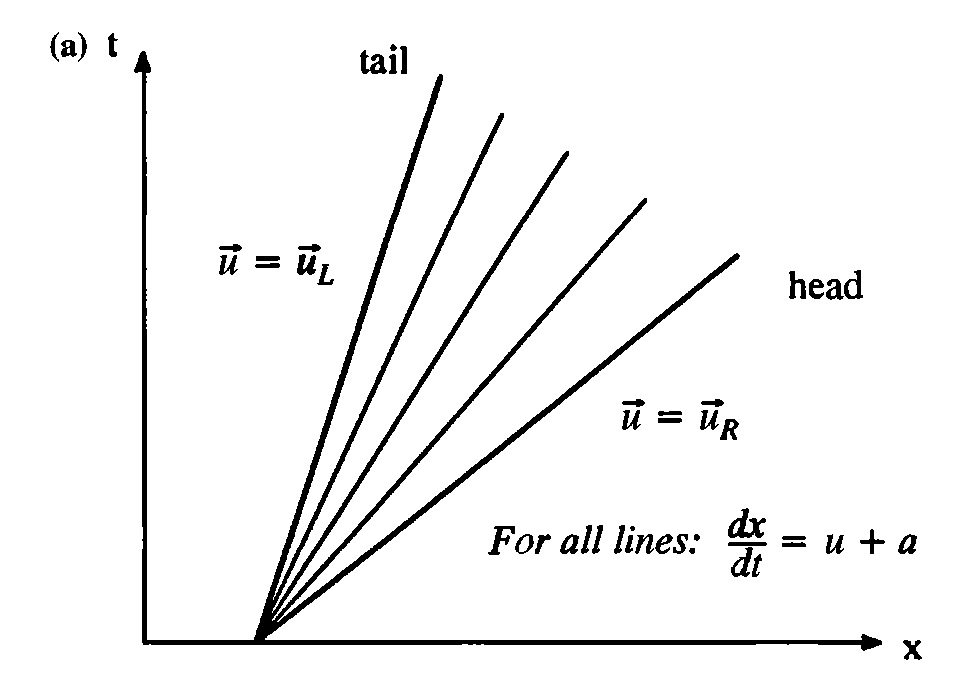
\includegraphics[scale=0.38]{figures/expansionfan1.jpg}
  \end{figure}
\end{frame}

\begin{frame}{EXPANSION WAVES}
  \begin{figure}
   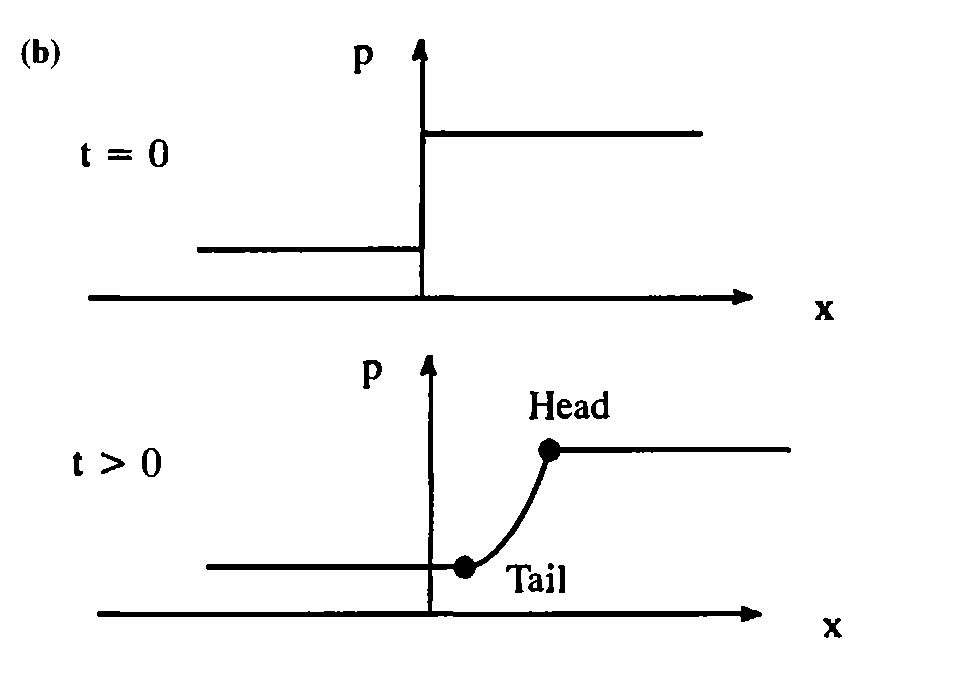
\includegraphics[scale=0.38]{figures/expansionfan2.jpg}
  \end{figure}
\end{frame}

\subsection{Compresion Waves and Shock Waves}

\begin{frame}{COMPRESION WAVES}
  \begin{itemize}
   \item It increases presure and density.
   \item In any region in which the wave speed $\lambda_2=u+a$ or $\lambda_3=u-a$ decreases monotonically from left to right. 
   \item Mathematically:
  \end{itemize}
  \begin{equation}
  \begin{matrix}
   u(x,t)+a(x,t)\geq{u(y,t)+a(y,t)}, & b_1(t)\leq{x}\leq{y}\leq{b_2(t)}\\
   or \\
   u(x,t)-a(x,t)\geq{u(y,t)-a(y,t)}, & b_1(t)\leq{x}\leq{y}\leq{b_2(t)}
  \end{matrix}
  \end{equation}
\end{frame}

\begin{frame}{SHOCK WAVES}
  \begin{figure}
   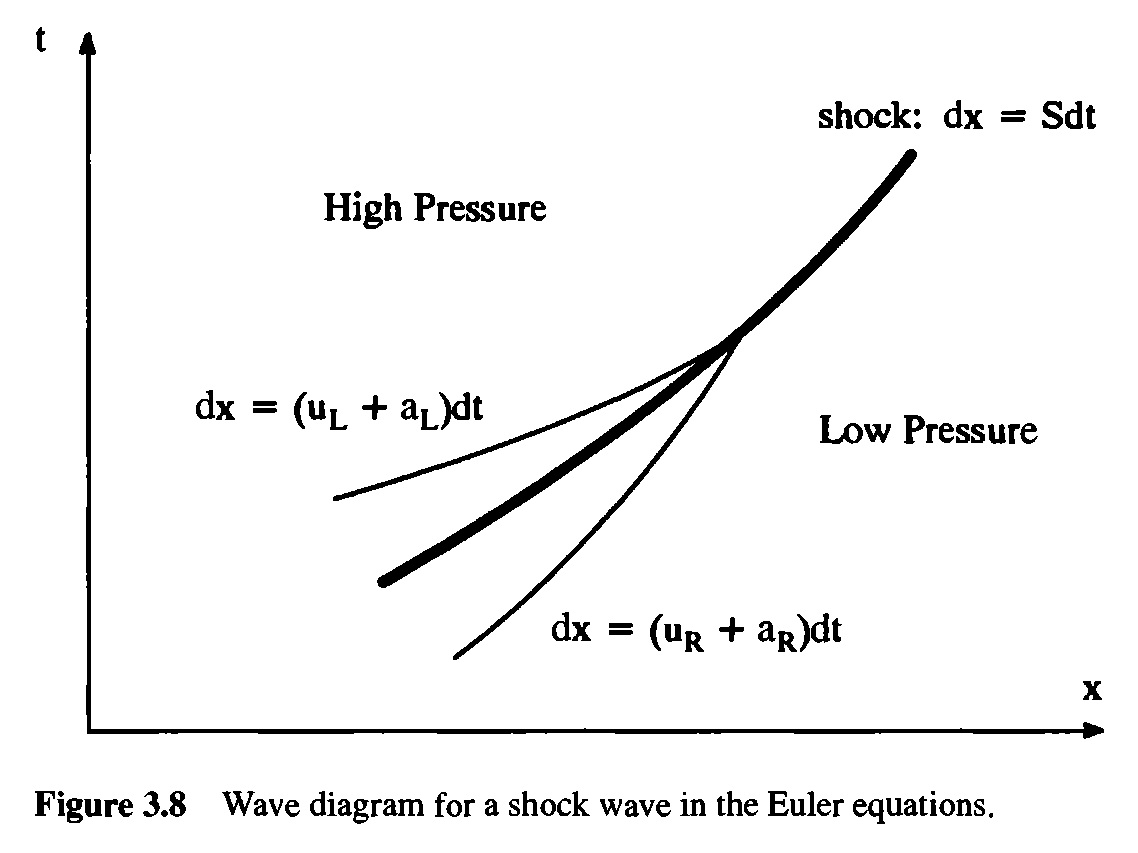
\includegraphics[scale=0.32]{figures/shockwdiag.jpg}
  \end{figure}
\end{frame}

\begin{frame}{SHOCK WAVES}
As we have seen:  
  \begin{itemize}
   \item The characteristics in a expansion diverge.
    \item The characteristics in a compresion diverge.
    \item An intersection between two or more characteristics from the same family creates a shock wave.
    \item A shock wave is jump discontinuity governed by Rankine-Hugoniot relations:
  \end{itemize}
    \begin{equation}
     \vec{f}_R-\vec{f}_L=S(\vec{u}_R-\vec{u}_L)
    \end{equation}
where:
  \begin{itemize}
   \item $\vec{f}_L,_R$ are flux vectors on the left- and right- side of the shock.
    \item $\vec{u}_L,_R$ are the conserved quantities on the left- and right- side of the shock.
  \end{itemize}
\end{frame}

\subsection{Contact Discontinuities}

\begin{frame}{CONTACT DISCONTINUITIES}
  \begin{itemize}
   \item Nearby Characteristics must diverge, converge or be precisely parallel each other. 
    \item Contact discontinuities are parallel entropy waves that neither create and compresion or expansion. They separate regions of different Entropy.
    \item They ocurr when $lambda_1=u$ and pressure are continuous while other flow properties jump. 
    \item In other words:
  \end{itemize}
  \begin{eqnarray}
    &&u_L=u_R,\\ 
    &&p_L=p_R
  \end{eqnarray}
\end{frame}

\begin{frame}{CONTACT DISCONTINUITIES}
  \begin{itemize}
   \item No fluid passes through a contact; thus the second law does not apply across a contact.
    \item  - Thus, entropy, density, energy, and all other other flow properties may either increase or decrease acrooss the contact.
    \item Like shocks, contacts discontinuities obey the Rankine-Hugoniot relations. 
    \item Unlike shock, contacts cannot form spontaneously: They must originate either in the initial condition or in the intersection of two shocks.
  \end{itemize}
\end{frame}

\section*{Waveforms Examples}

\begin{frame}{WAVEFORM EXAMPLE 1}
  \begin{figure}
   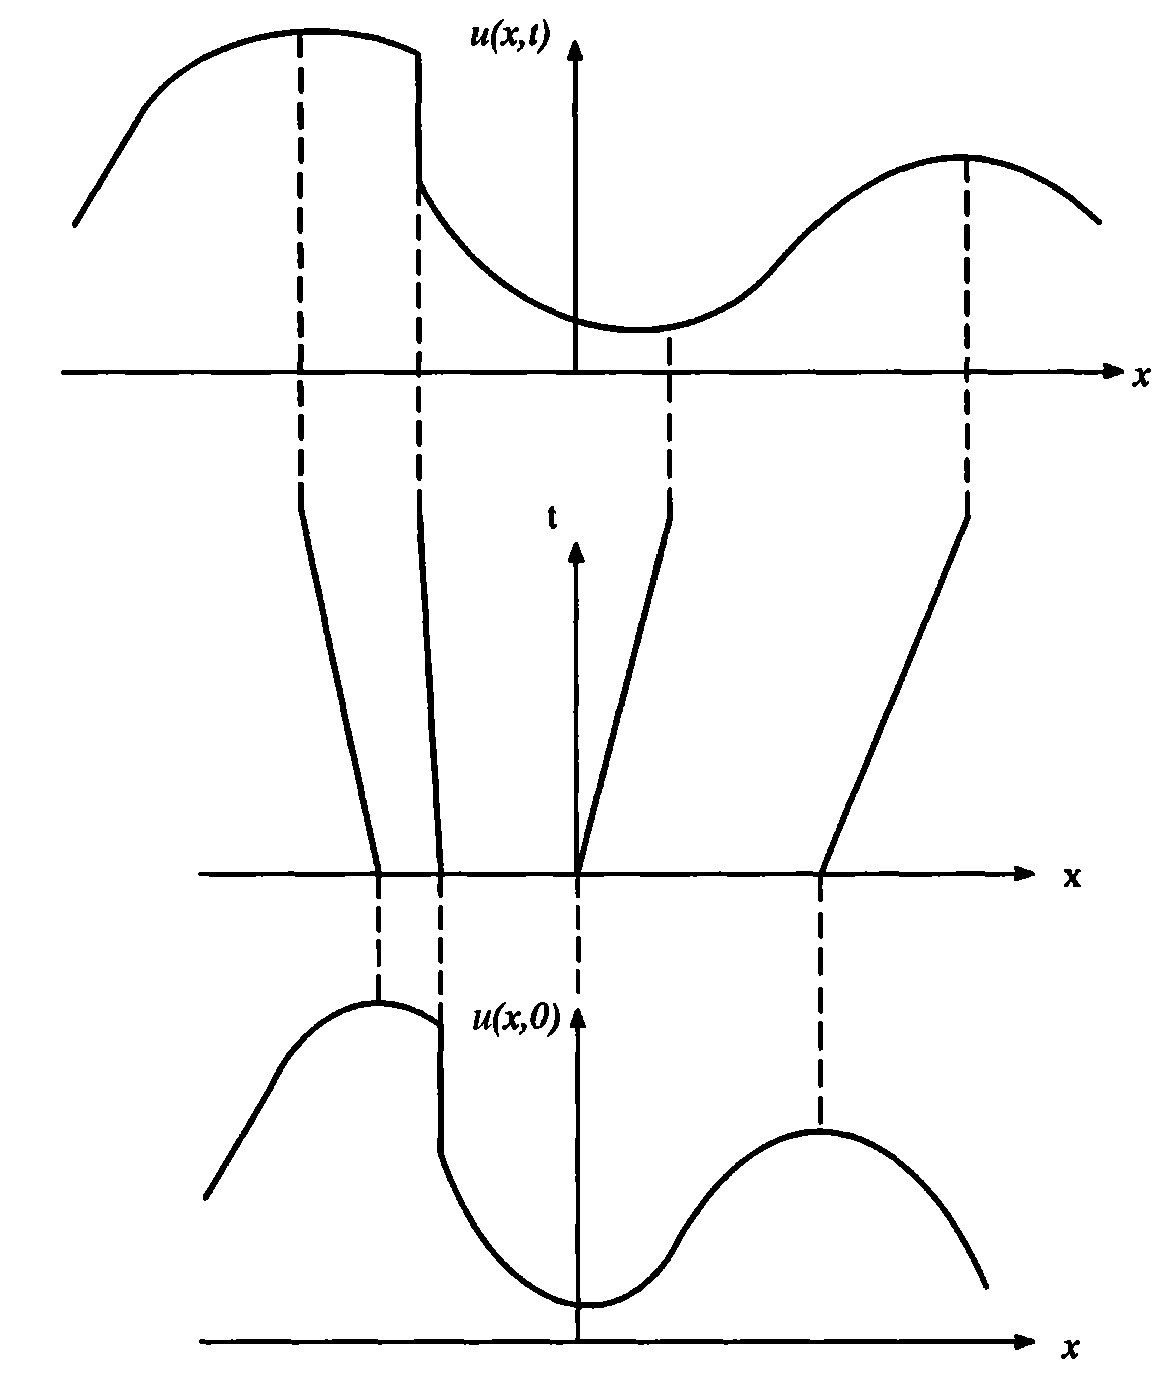
\includegraphics[scale=0.20]{figures/Preservation.jpg}
  \end{figure}
\end{frame}

\begin{frame}{WAVEFORM EXAMPLE 2}
  \begin{figure}
   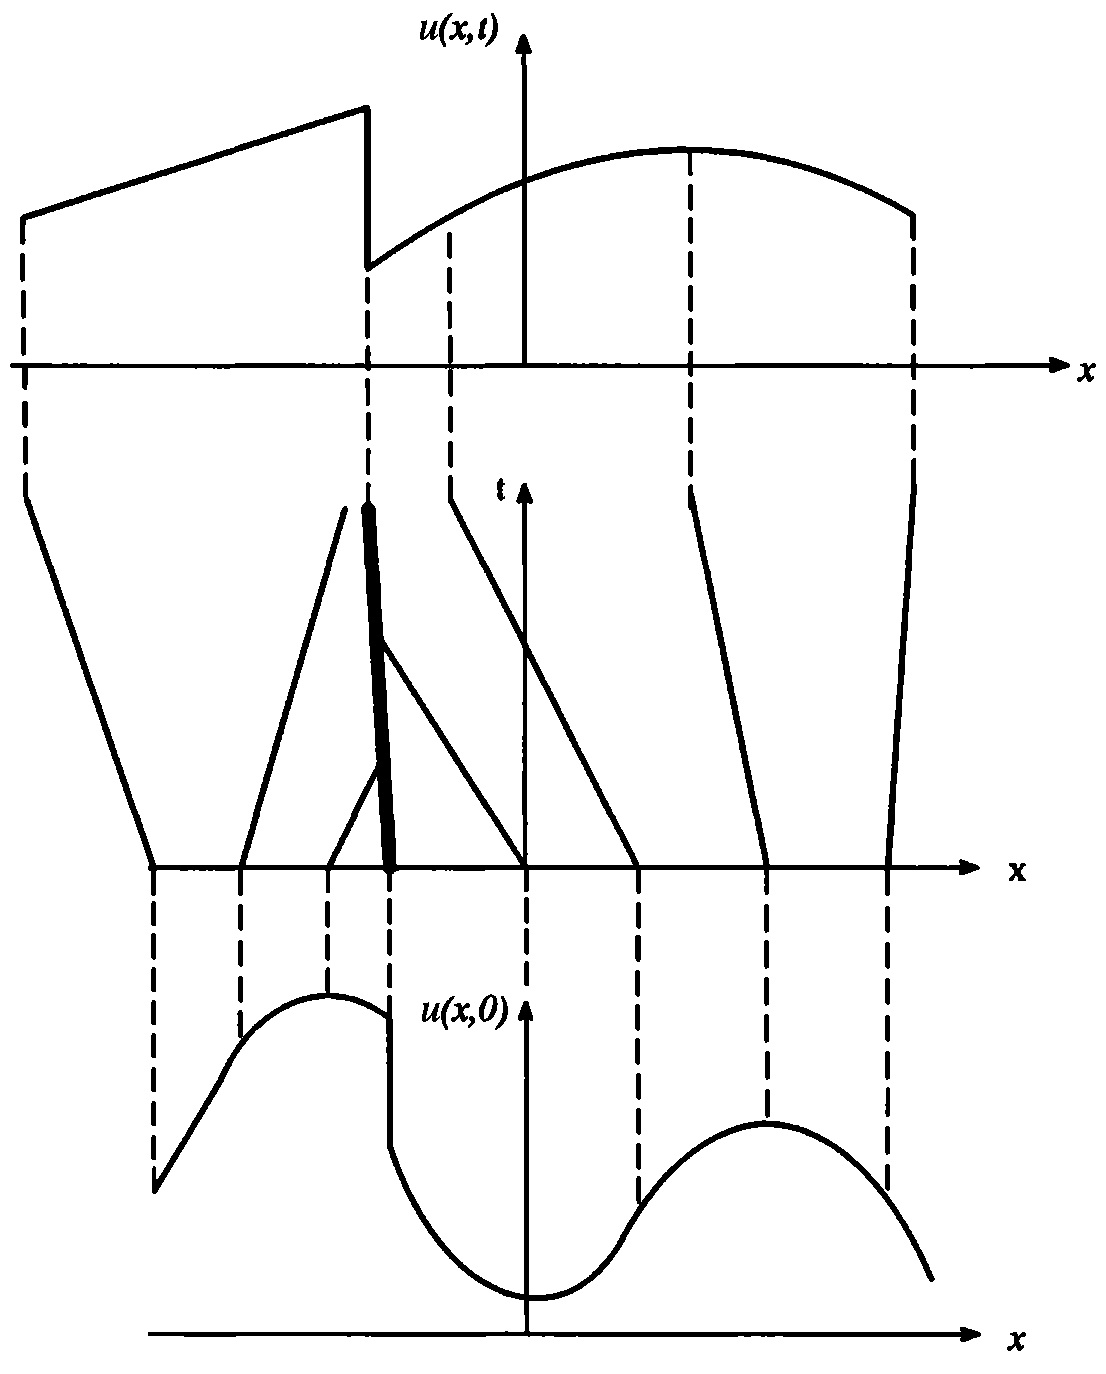
\includegraphics[scale=0.20]{figures/Destruction.jpg}
  \end{figure}
\end{frame}

\begin{frame}{WAVEFORM EXAMPLE 3}
  \begin{figure}
   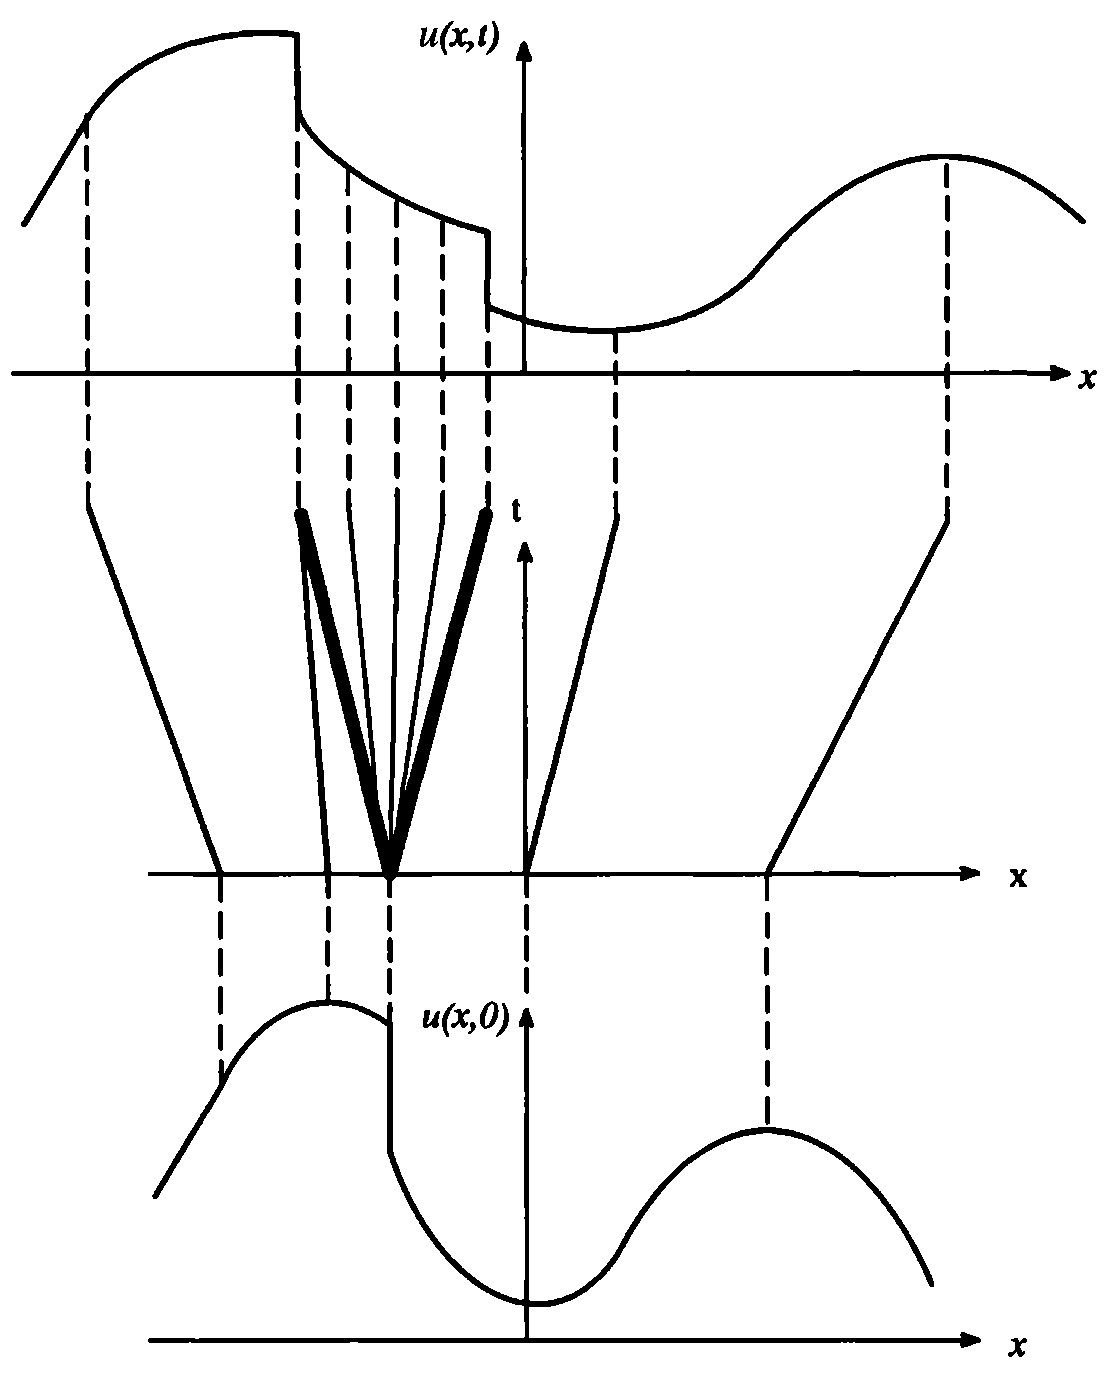
\includegraphics[scale=0.20]{figures/Creation.jpg}
  \end{figure}
\end{frame}

%\section*{Summary}

%\begin{frame}{Summary}

  % Keep the summary *very short*.
%  \begin{itemize}
%  \item
%    The \alert{first main message} of your talk in one or two lines.
%  \item
%    The \alert{second main message} of your talk in one or two lines.
%  \item
%    Perhaps a \alert{third message}, but not more than that.
%  \end{itemize}
  
  % The following outlook is optional.
%  \vskip0pt plus.5fill
%  \begin{itemize}
%  \item
%    Outlook
%    \begin{itemize}
%    \item
%      Something you haven't solved.
%    \item
%      Something else you haven't solved.
%    \end{itemize}
%  \end{itemize}
%\end{frame}


\end{document}


